\documentclass[11pt]{article}

\usepackage{acl2012}
\usepackage{times}
\usepackage{latexsym}
\usepackage{amsmath}
\usepackage{multirow}
\usepackage{url}

\usepackage{graphicx}
\usepackage{amsthm}
\usepackage{mathtools}
\usepackage{gnuplottex}

\usepackage{mystyle}

\usepackage[ps2pdf,unicode]{hyperref}   % Musí být za všemi ostatními balíčky

\DeclareMathOperator*{\argmax}{arg\,max}
\setlength\titlebox{6.5cm}    % Expanding the titlebox

\title{TrTok: A Fast and Trainable Tokenizer for Natural Languages}

\author{First Author \\
  Affiliation / Address line 1 \\
  Affiliation / Address line 2 \\
  Affiliation / Address line 3 \\
  {\tt email@domain} \\\And
  Second Author \\
  Affiliation / Address line 1 \\
  Affiliation / Address line 2 \\
  Affiliation / Address line 3 \\
  {\tt email@domain} \\}

\date{}

\begin{document}
\maketitle
\begin{abstract}
We present a data-driven tool for disambiguating token and sentence
boundaries. The implemented system is highly configurable and
versatile to the point its tokenization abilities allow to segment
unbroken Chinese text. The tokenizer relies on maximum entropy
classifiers and requires a sample of tokenized and segmented text as
training data. The system was built with multi-platform libraries only
and with emphasis on speed and correctness. After a necessary survey
of other tools for text tokenization and segmentation and a short
introduction to maximum entropy modelling, a large part of the paper
focuses on the particular implementation we developed and its
evaluation.
\end{abstract}

\section{Introduction}
\label{sec:introduction}

Tokenization and segmentation are parts of almost every natural
language processing system, since most of the higher-level language
processing applications assume we are dealing with words and
sentences, not with streams of bytes representing characters.


Segmentation (also referred to as sentence detection or sentence
boundary disambiguation) has been tackled using a variety of
techniques. The most common approaches include writing heuristics and
constructing abbreviation lists (the Stanford Tokenizer, the RE
system) or using machine learning algorithms to predict the role of a
potential sentence terminator (Satz, MxTerminator, Apache OpenNLP).
There have also recently been some very successful systems using
unsupervised methods (Punkt).

Tokenization is a problem which stops being trivial when we start
considering whitespace-free languages such as Chinese or Japanese. In
these languages, tokenization (also referred to as word segmentation)
receives a lot of attention \cite{seg-bakeoff}.

TrTok aims to be a practical tool for tokenizing and segmenting text
written in any language. To achieve such a goal, TrTok relies on the
user determining the specifics of training and tokenization and
providing the necessary training data.

TrTok's novelty comes in its openness and formalization of the
tokenization process. The process is divided into several discrete
stages, most of which are heavily customizable. The user is able to
say where in the text should TrTok consider breaking up or joining
tokens or sentences, how should TrTok represent the context of these
decision points to the underlying classifier, how should the
classifier be trained, how should existing whitespace be treated,
etc\ldots TrTok was also built to be a practical tool, which means it
can transparently process text interspersed with XML markup and HTML
entities and was designed to run fast.

The major inconveniences of TrTok are that due to its customizability
it needs to be properly set up and due to its reliance on machine
learning methods, it requires manually tokenized training data.
Furthermore, its dependency on external tools such as a build system
for automation of runtime code compilation can make it nontrivial to
deploy.

\section{Previous Work}
\label{sec:previous-work}

Established methods of sentence boundary disambiguation can be
organized into three distinct groups: rule-based systems, supervised
learning systems and unsupervised learning systems.

The \textbf{RE} system \cite{sbd-re} is an example of a rule-based
system. The program scans a document, looking for full stops. When one
is found, the word preceding it is compared to a list of regular
expression exceptions (mostly abbreviations) and unless the word is
found to match one of them, it is assumed to end the sentence. Besides
this core logic, the system also implements a small heuristic which
checks for numbers preceding the full stop and the word following it.

\textbf{MxTerminator} \cite{sbd-mxterm} is a supervised sentence
boundary disambiguator using maximum entropy models to predict whether
a potential sentence terminator does indeed signal the end of a
sentence. The prefix and suffix of the word containing the potential
sentence terminator and the words preceding and following it are
analyzed and their features are passed to the classifier. The features
consist of the tokens' type, their capitalization and their membership
status on a list of abbreviations which are either hand-prepared or
induced from data.

The biggest difference between TrTok and MxTerminator is that TrTok
does not assume any particular selection of features and thus offers
space for richer models (e.g., by extending the width of the context
or providing more complex features like part of speech tags).

An example of a system using more advanced features is the
\textbf{Satz} system \cite{sbd-satz}, which uses possible POS (part of
speech) tags as features in the machine learning algorithm.

Unsupervised learning systems are the most distinct from TrTok amongst
all the sentence boundary detection algorithms as they usually require
no manual configuration nor any training data to function properly. A
great example of an unsupervised sentence boundary disambiguator is
the \textbf{Punkt} system \cite{sbd-punkt}.

Punkt relies mostly on collocation detection techniques but also makes
use of an orthographic heuristic to analyze the test data in several
passes and disambiguate abbreviations and sentence terminators. The
system has shown remarkable performance without needing any manual
tuning or training data.

\section{Description of the System}
\label{sec:system}

TrTok is implemented by a parallel execution of several configurable
pipeline steps. This pipeline can be repurposed to train the embedded
classifier using tokenized data, to tokenize new data using a trained
classifier and to evaluate the predictions of a trained classifier on
manually tokenized data.

We will describe the important pipeline steps one by one, in the order
in which they process data when tokenizing new text.

\subsection{RoughTokenizer}

The RoughTokenizer partitions the stream of input characters into
small, discrete chunks of non-blank characters called \newterm{rough
tokens}. The partitioning can be made more granular by user-defined
rules which specify positions at which the desired tokenization might
differ from the whitespace-induced one.

A location in the text may be marked as a \maysplit{} meaning that the
characters in the text preceding and following it may be parts of
different tokens even though they are not separated by whitespace
(e.g. we might wish to put a \maysplit{} between \example{``was''} and
\example{``n't''} in \example{``wasn't''}).

A location within a span of white characters might be labeled as a
\mayjoin{} signalling that the characters preceding and following the
whitespace area might be parts of the same token, as in the case of
spaces entered in long numbers for readability (e.g.
\example{``12~345''}).

Finally, a location in the text may be marked as a \maybreaksentence{}
if the characters preceding it and the characters following it might
belong to different sentences.

\begin{figure}
  \begin{center}
    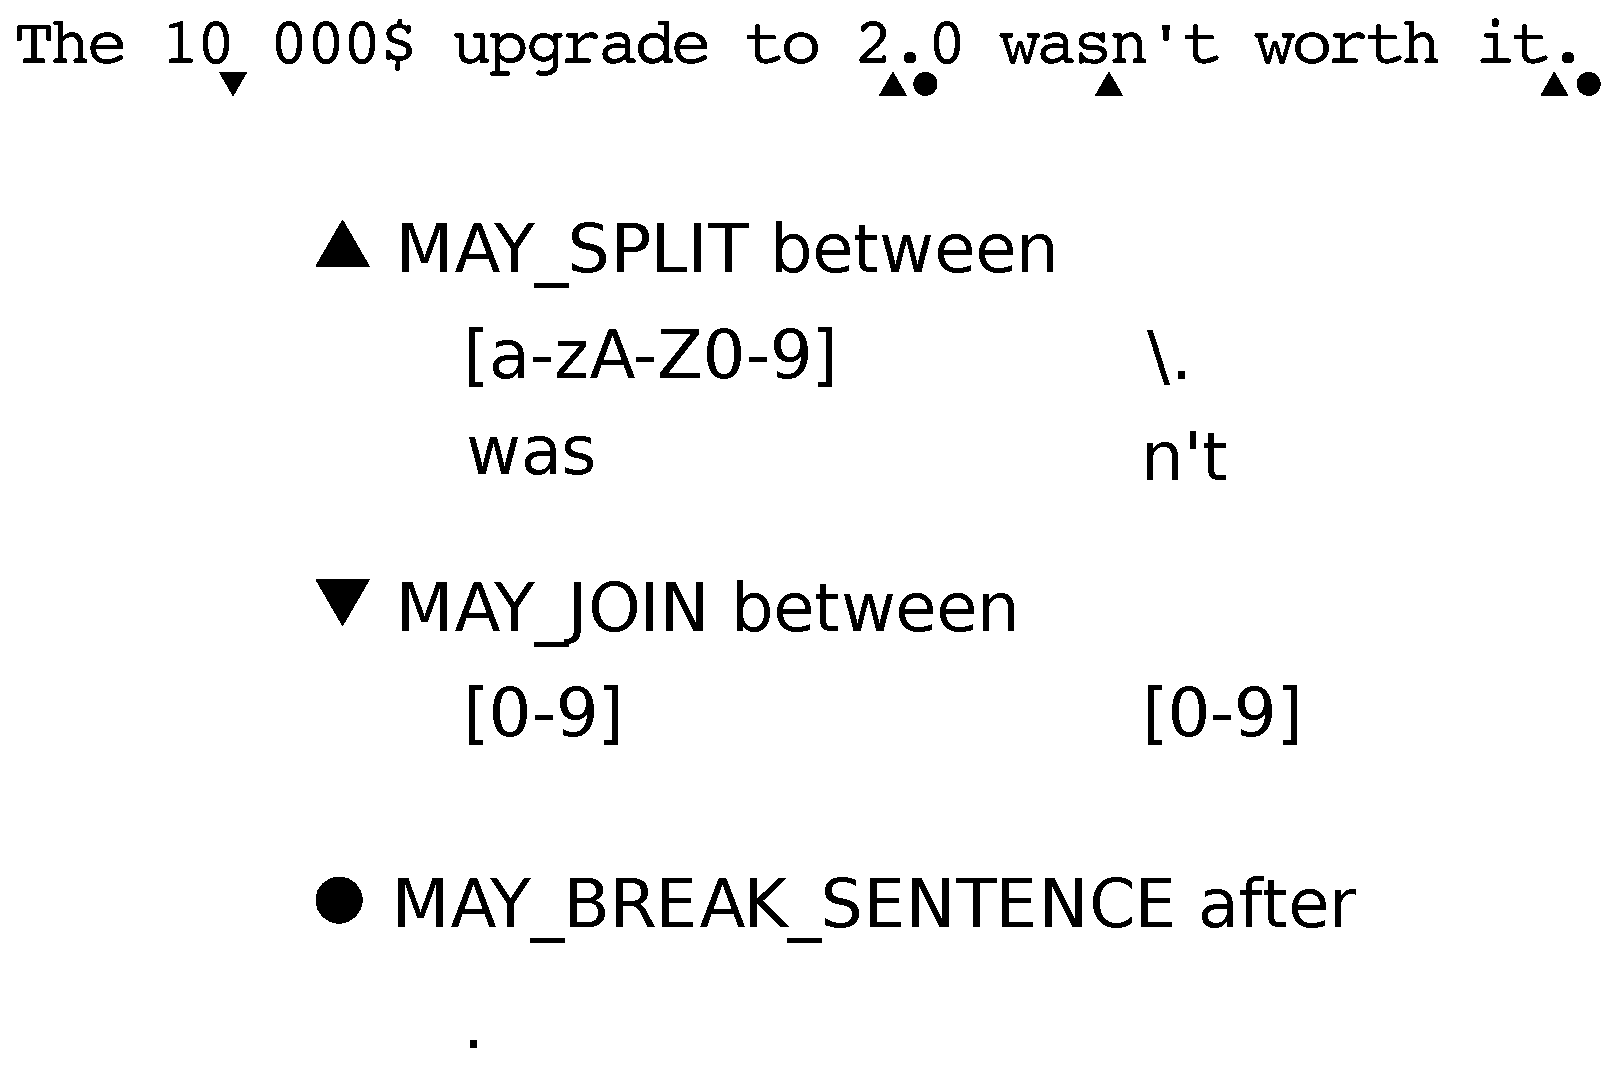
\includegraphics[width=\textwidth / 2]{img/decisionpoints.eps}
    \caption{In this example, $\blacktriangle$ stands for \maysplit{},
      $\blacktriangledown$ for \mayjoin{} and $\bullet$ for
      \maybreaksentence{}. This is how the rough tokenization might
      turn out given some reasonable settings for tokenizing English.}
    \label{fig:decision-points}
  \end{center}
\end{figure}

See Figure~\ref{fig:decision-points} for an example of how these
potential tokenization operations can look like in one sentence. A
rough token is defined as a maximal sequence uninterrupted by
whitespace or a possible tokenization operation (the symbols
underneath the sentence in Figure~\ref{fig:decision-points}). For
example, in the sentence from Figure~\ref{fig:decision-points},
``was'', ``n'', the apostrophe and ``t'' are all individual rough
tokens. Note that the presence of a \may{} event only signifies the
possibility of a tokenization operation (splitting or joining of
tokens or sentences). Whether a token split, token join or sentence
break will occur is up to the Classifier.

The locations of these possible tokenization operations are determined
by user-defined rules which each consist of a pair of regular
expressions. The respective tokenization operation is signalled if the
characters leading up to and following a position match the regular
expressions in one of these rules.

If we look back at Figure~\ref{fig:decision-points}, we might imagine
more robust settings also placing a \maybreaksentence{} after the
apostrophe/single quote, while others might be more daring and not
place a \maybreaksentence{} after the point in ``2.0'', because it is
followed by a non-blank character.

TrTok collects these rules and generates a Quex program implementing a
fast FSM, which gets compiled and loaded in
(Quex\footnote{http://quex.sourceforge.net} is a fast and more
Unicode-friendly variation on the classic tools lex and flex for C++).

\subsection{FeatureExtractor}

The stream of rough tokens interleaved with potential tokenization
operations output by the RoughTokenizer is processed using the
FeatureExtractor. The FeatureExtractor annotates each rough token with
a bit vector signifying which of the user-defined feature predicates
hold for the rough token in question.

The features can be defined in two ways: either using a regular
expression or a list of rough tokens. For a feature defined using a
regular expression, a rough token is said to have that feature if and
only if the regular expression matches the entire rough token. In the
case of a feature defined using a list of rough tokens, a rough token
is said to have that feature if and only if it is on the list.

This way it is easy to specify features which try to analyze the shape
of rough tokens using regular expressions or to simply give a list of
all interesting tokens (e.g. words of a certain part of speech or
exceptions such as abbreviations).

\subsection{Classifier}

The Classifier is the other busy element in the pipeline (besides the
RoughTokenizer). Its job is to disambiguate the potential tokenization
operations identified by the RoughTokenizer, i.e. it decides whether a
\maysplit{} truly splits a word into two tokens, whether a \mayjoin{}
truly joins two words into one token and whether a \maybreaksentence{}
truly ends a sentence. It does so by consulting a maximum entropy
classifier for every location containing these potential tokenization
operations.

The features passed to the classifier consist of the features of rough
tokens in the context surrounding the potential tokenization operation
and the presence of whitespace and potential tokenization operations
in the context area. The user is free to select the size of the
context area and which features from which rough tokens in the context
area should be passed to the classifier.

Features can also be clustered together into conjunct features which
provide a value for every combination of the constituent features'
values (this lets the trainer estimate a different parameter for
different combinations of the features' values, which is useful to
model the joint influence of some features).

The classifier then marks each location with a potential tokenization
operation as either a sentence boundary, token boundary or no boundary
(meaning the location is inside a token). Using this classification,
any potential tokenization operations are finally disambiguated.

\subsection{OutputFormatter}

The OutputFormatter is the point at which the stream of rough tokens
is turned back into a character stream. This means that all the rough
tokens are concatenated and whitespace is inserted between them
depending on whether there originally was any whitespace between them
and on the tokenization operations which are to be carried out in the
space between them. Individual tokens end up being separated by a
single space character and sentences are separated by line breaks.

\section{Evaluation}
\label{sec:eval}

We evaluated our implementation of TrTok compared to a wide range of
prominent implementations and approaches to sentence detection. The
results are given in Table~\ref{tbl:grand-melee}.

\subsection{Dataset}

The experiments were conducted on the Brown corpus \cite{data-brown}
as supplied through NLTK \cite{software-nltk}. A representative
(covering each category of text proportionately) 20\% of the corpus
was used as the testing data. This number was chosen so that the
testing data would be sure to contain at least 1,000 instances of a
non-sentence-terminating full stop; the resulting test set ended up
containing 1,481 such full stops. The rest of the data was made
available for training to the supervised learning methods.

\subsection{Performance Measurement}

The performance of the evaluated systems was measured by their success
(accuracy) in classifying instances of the full stop character. The
text contains other sentence terminators such as the question mark and
the exclamation mark, but they almost never serve as anything else but
sentence terminators in the text. Other occasional sentence delimiters
such as dashes, semicolons, colons and line breaks were ignored as
well, since the other systems usually do not have a solution for them.
This way, the comparison is fair. Furthermore, the full stop is the
most common and ambiguous of the sentence delimiters, so it makes
sense to focus on it.

Besides the systems' accuracy, we also measure the time spent for
processing the whole testing data and we present the median of 11 runs
to bring the implementation speed of the systems into consideration as
well.

\subsection{Sentence Detection Methods}

\begin{table}
  \small
  \begin{center}
    \begin{tabular}{ | l | c | c | c | c | c | r | }
      \hline
      & Acc. $\downarrow$ & Err. Rate & Prec.
      & Recall & F_1 & Time \\ \hline
      TrTok::Groomed & \textbf{98.86\%} & \textbf{1.14\%} & \textbf{99.12\%}
                     & 99.57\% & \textbf{99.34\%} & 5.10s \\ \hline
      Stanford CoreNLP & 98.83\% & 1.17\% & 98.78\%
                       & 99.89\% & 99.33\% & 5.02s \\ \hline
      TrTok::MxTerm-like & 98.76\% & 1.24\% & 98.70\%
                         & 99.89\% & 99.29\% & 1.10s \\ \hline
      TrTok::Easy & 98.70\% & 1.30\% & 98.61\%
                  & 99.91\% & 99.26\% & 1.08s \\ \hline
      Punkt & 98.65\% & 1.35\% & 98.82\%
            & 99.63\% & 99.22\% & 3.13s \\ \hline
      MxTerminator & 98.27\% & 1.73\% & 98.30\%
                   & 99.74\% & 99.01\% & 1.37s \\ \hline
      Apache OpenNLP & 98.20\% & 1.80\% & 98.20\%
                     & 99.77\% & 98.97\% & 1.13s \\ \hline
      Apache OpenNLP (ready) & 97.71\% & 2.29\% & 98.62\%
                             & 98.75\% & 98.68\% & 1.17s \\ \hline
      RE & 97.26\% & 2.74\% & 98.52\%
         & 98.32\% & 98.42\% & 16.93s \\ \hline
      TrTok::Satz-like & 96.50\% & 3.50\% & 97.91\%
                       & 98.08\% & 97.99\% & 1.59s \\ \hline
      TrTok::Baseline & 91.84\% & 8.16\% & 91.67\%
                      & 99.66\% & 95.50\% & 0.85s \\ \hline
      Absolute Baseline & 86.89\% & 13.11\% & 86.89\%
                        & \textbf{100.00\%} & 92.99\% & \textbf{0.02s} \\ \hline
    \end{tabular}
  \end{center}
  \caption[Performance of sentence detectors on the Brown corpus] {The
    performance of the various sentence detectors on full stops from
    the Brown corpus testing data. The 1.15 MB of testing data
    consisted of 11,376 sentences and 232,893 tokens.}
  \label{tbl:grand-melee}
\end{table}

\textbf{Absolute Baseline} simply marks every full stop as a sentence
terminator.

\textbf{Trtok::Baseline} is the simplest tokenizer which can be
written in TrTok. However, even the simplest TrTok configuration
always uses the whitespace following the possible tokenization
operation as a feature and thus it is able to perform better than the
Absolute Baseline.

\textbf{TrTok::Satz-like} is a straightforward attempt at
reconstructing the Satz system in TrTok. The POS-tagged training data
was used to construct lexicons for each different part of speech tag
(NLTK's method of simplifying tags was used to reduce the number of
different tags to overcome data sparsity). The POS tags for three
tokens on either side of the full stop were used as the features.

TrTok::Satz-like's system of tags is not as refined as the original
and it does not use its fallback regular expression heuristics and
hence it does not perform as well as the original Satz system did
\cite{sbd-satz}.

The \textbf{RE} system, \textbf{MxTerminator} and \textbf{Punkt} were
described in Section~\ref{sec:previous-work}. For training, Punkt
received the entire Brown corpus (training data and testing data)
without any annotations while MxTerminator was trained using the
training data.

Punkt achieves remarkable performance and stands as the strongest
competitor to TrTok in the field of multilingual sentence detection.
They are both accurate language-independent tools but TrTok's big
shortcoming is its need for a corpus of manually tokenized data.

\textbf{Apache OpenNLP} contains a sentence detector based around a
maximum entropy classifier. The implementation is nearly identical to
the specification of MxTerminator with only minor deviations (such as
signalling surrounding whitespace as features).

We performed experiments both with the ready-made model for English
distributed via OpenNLP's website and with a model which was trained
on our training data.

The \textbf{Stanford CoreNLP} sentence splitter works by applying its
tokenizer to the input text which makes the distinction between a full
stop as part of an abbreviation or an ordinal number as opposed to a
full stop as a sentence terminator. Thus the task of sentence
splitting is trivial after the tokenization has been performed. The
tokenizer is a rule-based program implemented using a lexical analyzer
generator, JFlex (similar to how TrTok uses Quex to implement the
RoughTokenizer).

The Stanford Tokenizer's performance is excellent, especially
considering it has not had the chance to train itself on the target
corpus. However, the Stanford Tokenizer is written explicitly for
English and it is likely that its performance would not carry over to
other languages without significant work.

\textbf{TrTok::MxTerm-like} is a reconstruction of MxTerminator in
TrTok. It is a nice demonstration of the ease with which new
tokenization setups can be defined in TrTok. The entire setup
consisted of creating a directory, collecting the abbreviations in a
single file and writing five lines of configuration, two or three of
which could be easily obsoleted by adopting saner defaults in TrTok
and one of which is purely for convenience.

The reason why MxTerminator does not achieve the same performance
could be that the maximum entropy trainer used in MxTerminator limits
itself to 100 iterations of Generalized Iterative Scaling, which
converges very slowly compared to L-BFGS \cite{maxent-algorithms}.
Another reason might be the fact that both MxTerminator and OpenNLP
cut off infrequent features.

The high accuracy of TrTok::MxTerm-like led us to try and see what
happens when we simplify the tokenization setup even further, which
led to \textbf{TrTok::Easy} which works the same way as
TrTok::MxTerm-like, but which does not use any abbreviation lists,
merely the token types surrounding the full stop. Therefore,
TrTok::Easy does not rely on any external linguistic knowledge and is
fairly language universal, given that we have enough training data.
The performance of TrTok::Easy also points out that the difference in
performance between TrTok and MxTerminator/OpenNLP cannot be explained
by the different abbreviation lists.

Finally, \textbf{TrTok::Groomed} is a large, hand-made tokenization
setup ported from a previous version of the tokenizer. It considers 24
different potential sentence terminators, it includes seven distinct
lists of abbreviations totalling 303 types (prefix and suffix titles,
abbreviated names of months, etc.) and it implements features for
detecting the case of tokens, for noticing numbers which happen to be
in the range of years, or the days of the month, etc\ldots\ \ These
features are extracted from rough tokens within eight tokens distance
from the full stop. The two closest tokens on either side of the full
stop also contribute their token type as a feature.

Due to the large number of potential tokenization operations and
user-defined features, TrTok::Groomed's speed lags significantly
behind the other TrTok setups.

Interestingly, there is not much difference in the performance of
TrTok::Groomed, TrTok::MxTerm-like and TrTok::Easy. This tells us that
besides the token types in the close vicinity of the full stop, other
features are not that important. This highlights another use for TrTok
as a tool for the fast analysis of the importance of different
contextual features for performing the task of sentence detection.

\subsection{Chinese Word Segmentation}

Since TrTok is a general program for splitting text into sequences
(sentences) which are in turn composed of other sequences (tokens)
based on user-defined features, TrTok can be used for more than just
sentence detection. One other segmentation task we had hoped might be
solvable using TrTok is Chinese word segmentation.

We ported the key features of one of the top contestants (which also
happens to employ a maximum entropy classifier)
\cite{seg-chinese-maxent} in the 2005 Second International Chinese
Word Segmentation Bakeoff into TrTok and evaluated its performance
using the official evaluation scripts. The results achieved (see
Table~\ref{tbl:bakeoff-score}) are approximately a median of the
scores reported for submissions to the Bakeoff.

\begin{table}
  \small
  \begin{center}
    \begin{tabular}{ | l | r | r | r | r | }
      \hline
      & True Words Recall & Test Words Precision & F-measure \\ \hline
      Academia Sinica & 0.933 & 0.919 & 0.926 \\ \hline
      City University & 0.934 & 0.934 & 0.934 \\ \hline
      Peking University & 0.923 & 0.933 & 0.928 \\ \hline
      Microsoft Research & 0.951 & 0.952 & 0.951 \\
      \hline
    \end{tabular}
  \end{center}
  \caption[Chinese Word Segmentation scores]
    {The scores assigned to our tokenizer by the official scoring script of the
    Second International Chinese Word Segmentation Bakeoff, sorted by dataset.}
  \label{tbl:bakeoff-score}
\end{table}


\section{Conclusion}
\label{sec:outro}

Placeholder.


\bibliographystyle{acl2012}
\bibliography{sbd,maxent,seg,web}

\end{document}
